\chapter{Literature Review}

Once upon a time engineers and researchers believed... In this area of research, they used the following methods... \cite{jct2010}

Write this section first as it will take you the longest. I suggest you start writing this as soon as you
have done your initial research at the beginning of your project. You can then return to it once you
have completed your work to edit and adjust it.

A literature review forms the theoretical basis of your project. You need to read a large number of
journal papers, sections in books, technical reports etc. relevant to your work at the start of project.
This will give you a good idea of the field of research.

When writing your review start of with the general concepts and move to the more specific aspects
explaining the necessary theory as you go. This section is NOT a copy and paste from others work or a
rewrite-but-change-one-word section. I suggest you read all your material, and then put it down and
write this section, referring back to the work only when you need to check something.

See your PCS textbook for more details on how to write a literature review.

If you include a figure or a table in your text please see the example in Fig. \ref{fig:model} as to how to caption it.
Please make sure that all text in your figures is readable and that you reference your figures if they are
from another source.

\begin{figure}[ht]
\centering
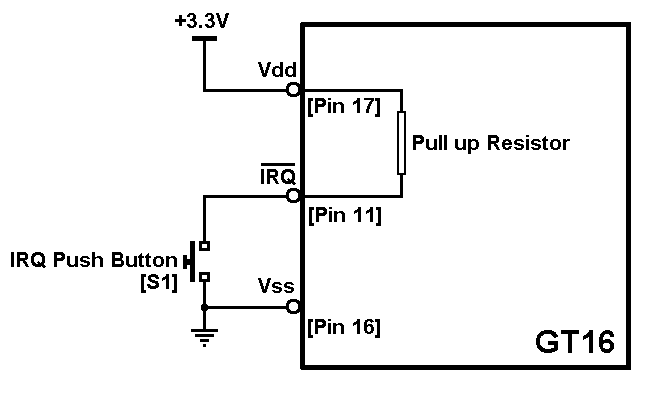
\includegraphics[width=0.7\textwidth]{model.png}
\caption{A block diagram illustrating the connections to the IRQ pin on the MCS08GT16A microcontroller (Please
note that your headings should be short descriptions of what is in the diagram not simply the figure title)}
\label{fig:model}
\end{figure}
\section{Gait sequence modelling and estimation}
\subsection{Quadrupede gait modelling}
\subsubsection{Periodicity}
\subsection{Quadrupede gait estimation}
\section{Case study: Inertia Measurement Unit}
\section{Hidden Markov Models}
Hidden Markov Models (HMMs) are doubly embedded stochastic processes with a rich underlying statistical structure. Introduced at the end of the 1960s by Baum and colleagues, they have become one of the prefered techniques in speech recognition after the implementation of Baker and Jelinek in 1970s. HMMs have been successfully applied to various other engineering problems in pattern recognition for classification and fraud detection purposes, amongst others.
%%TODO: ref: A tutorial on hidden Markov models and selected, Tool wear condition monitoring in drilling operations using, and Two-phase flow pattern identification using continuous hidden Markov model hidden Markov models (HMMs)

\subsection{HMM parameters specification}
An HMM is fully specified the following parameters 
\begin{enumerate}
	\item N, the number of distinct states of the model. Together they form the set of individual states \(S = \{S_1, S_2, ..., S_N\}\).
	\item T, the number of observations. A sample observation sequence is denoted as \(O = \{O_1, O_2, ..., O_T\}\).
	\item \(Q = {q_t}\), the set of states with \(q_t\) denoting the current state at time instance, t such that \(q_t \epsilon S\) and \(t = 1, 2, ..., T\).
	\item K, the number of distinct observation symbols per state. 
	\item \(V = \{v_1, v_2, ..., v_K\}\), the feature set of K dimensions.
	\item \(A =  \{a_{ij} \}\), the state transition probabilities. It \(a_{ij}\)  denotes probability of transitioning from state \(S_i\) to state \(S_j\).
	\item \(\Phi =   \{ \phi_{j}(k\}\), the probability distribution of observation symbols in state j.
	\item The initial state distribution, \(\pi = \pi_i\)
\end{enumerate}
For continuous HMM (CHMM), i.e, HMM with continuous-valued observations, \(\Phi\) consists in a probability distribution function. Many applications have continous distributions with mixtures of Gaussian distribution. %%TODO: quote
As such, \(\phi\) is approximated by a weighted sum of M multivariate Gaussian distributions \(\eta\),

\begin{align} \label{eq:mix}
	\phi(O_t) = \sum_{m=1}^M \beta_{jm} \eta(\mu_{jm}, \Sigma_{jm}, O_t), \\
	\eta(\mu, \Sigma, O) = \frac{1}{\sqrt{(2\pi)^K|\Sigma|}}exp(-\frac{1}{2}(O-\mu)'\Sigma^{-1}(O-\mu)
\end{align} 
\begin{align*}
	1 \leq j \leq N; 1 \leq m  \leq M; \beta_{jm} \geq 0; \sum_{m=1}^{M}\beta_{jm} = 1
\end{align*}
where \(\beta_{jm}\) is the mixture composition coefficient; \(\mu_{jm}\), \(\Sigma_{jm}\), respectively the mean vector and covariance matrix of state j; M is the number of mixture components and K is the dimensionality of O.

Thus, the compact specification of a continous valued observation HMM defined in \ref{eq:CHMM} and that of a discrete HMM in \ref{eq:DHMM}.
\begin{align} 
	\alpha = (A, \beta_{jm}, \mu_{jm}, \Sigma_{jm}, \pi) \label{eq:CHMM} \\
	\alpha = (A, b_j(k), \pi) \label{eq:DHMM}
\end{align}

\subsubsection{Basic assumptions of HMMs theory}
HMM theory is built on three basic assumptions listed below. They not only, make it a relatively simple graphic modelling tool but, also simplify its implementation. This naturally comes with some limitations in modelling more complex problems, which however, may be modelled with higher order HMMs. %%Quote
\begin{enumerate}
\item \textit{The Markov assumption}: HMM assumes that the probability of being in the current	at any instance of time t, is uniquely dependent on the previous state, at time, t + 1. More specifically, \(a_{ij} = P[q_t = S_j|q_{t+1}=S_i]\). This assumption makes it unsuitable for long-range correlation capturing applications.
\item \textit{The stationary assumption}: Furthermore, HMM state transition probabilities are assumed to be time-independent. Thus, the transition probabilities of two distinct time, \(t_1\) and \(t_2\) are identical, \(P[q_{t_1} = S_j|q_{t_1 -1} = S_i] = P[q{t_2}=S_i|q_{t_2-1} = S_i]\). HMMs can therefore effectively model mechanisms with stationary observations.
\item \textit{The output/observation independence assumption}: The current observation also known as emission symbol is statistically independent of the previous observations. It is "emitted" only by the current state, \(P[O|q_1, q_2, ..., q_T, \alpha]=\prod_{t=1}^{T}P[O_t|q_t, \alpha]\).
\end{enumerate} 
The above three assumptions are similar to those of a Markov chain. This is because the stochastic process of an HMM pertaining to the hidden states can be reduced to a Markov chain. Thus, the essential difference between an HMM and a Markov process is that with the former there is not a one-to-one correspondence between the states and the symbols. %%TODO: Quote biology book

\subsection{Three fundamental problems for HMM design}
In %%TODO: quote: A tutorial on Hidden Markov
, Lawrence stipulates an HMM design needs to answer three fondamental problems. The three problems and their solutions are discussed in the next sub-sections. 

\subsubsection{The training problem}
\subsubsection{The evaluation problem}
\subsubsection{The decoding problem}

\subsubsection{First order Markov model - current and predecessor only considered}

\subsection{Types of HMM}
\subsubsection{Ergodic model}
\subsubsection{Left-Right model or Bakis model}
\subsubsection{Evaluation of the probability of a sequence of observations}
\subsubsection{The determination of a best sequence states}
\subsubsection{The adjustment of model parameters to account for observed signal}
\section{k-Nearest Neighbour}
\section{Dimension reduction}
\subsection{Feature selection}
\section{Sufficiency of Training Data}
\section{Techniques to increase Training Data}
\subsection{Mirroring}